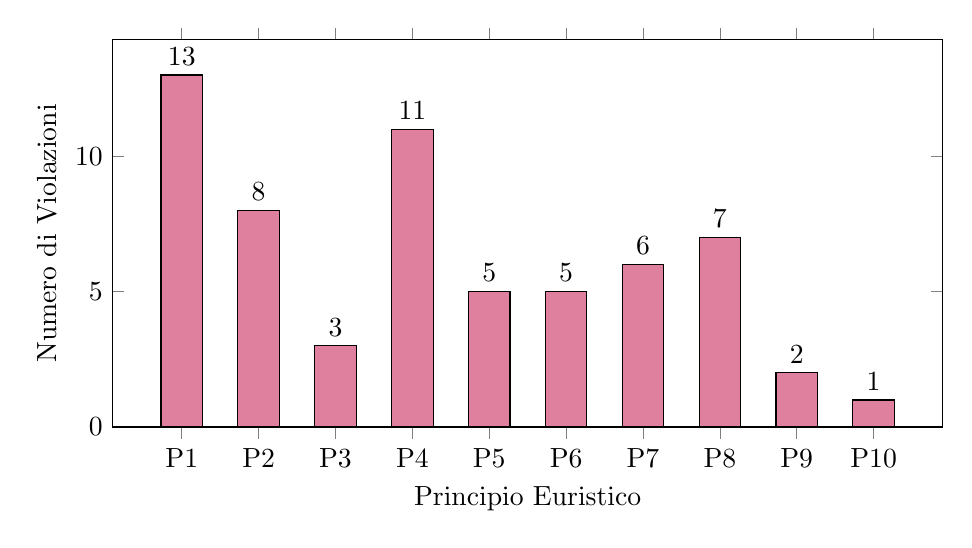
\begin{tikzpicture}
    \begin{axis}[
        ybar,
        bar width=15pt,
        enlarge x limits=0.1,
        ylabel={Numero di Violazioni},
        xlabel={Principio Euristico},
        symbolic x coords={P1, P2, P3, P4, P5, P6, P7, P8, P9, P10},
        xtick=data,
        nodes near coords,
        nodes near coords align={vertical},
        width=\textwidth,
        height=6.5cm,
        ymin=0
    ]
        \addplot[fill=purple!50] coordinates { (P1,13) (P2,8) (P3,3) (P4,11) (P5,5) (P6,5) (P7,6) (P8,7) (P9,2) (P10,1) };
    \end{axis}
\end{tikzpicture}